\titre{Optimisation simple}
\theme{Optimisation}
\auteur{Jean-François Culus}
\organisation{AMSCC}
\contenu{

\texte{On considère la fonction $f$ définie sur $\mathbb{R}^2$ par 
$$ f(x,y)= (x^2+y^2) e^{-x}$$
}

\begin{enumerate}
\item 
\question{ Justifier (rapidement) que cette fonction est de classe $\mathcal{C}^2$ sur $\mathbb{R}^2$. }
\reponse{ Les fonctions $(x,y)\mapsto x^2+y^2$ et $(x,y)\mapsto e^{-x}$ étant de classe $\mathcal{C}^{\infty}(\mathbb{R}^2)$,  leur produit l'est aussi. }

\item
\question{Trouver les points critiques de $f$ sur $\mathbb{R}^2$.}
\reponse{Calculons déjà les dérivées partielles premières de $f$. Nous avons: 
\\ $\frac{\partial f}{\partial x} (x,y)=2x e^{-x} -(x^2+y^2) e^{-x}$
$\frac{\partial f}{\partial y} (x,y)= 2y e^{-x}$. 
\\ Ainsi, cherchons les valeurs $(x,y) \in \mathbb{R}^2$ telles que 
$$ \frac{\partial f}{\partial x}(x,y) = \frac{\partial f}{\partial y}(x,y) =0$$
De $\frac{\partial f}{\partial y}(x,y)=0$, nous déduisons que $y=0$ et en injectant dans l'autre équation, nous obtenons que $2x -x^2=0$ soit $x(2-x)=0$ et donc $x=0$ ou $x=2$.
\\ Les points critiques sont alors $(0,0)$ et $(2,0)$. }

\item
\question{Trouver les extrema locaux de $f$ sur $\mathbb{R}^2$.}
\reponse{ Etudions les dérivées secondes de $f$: 
\\ $\frac{\partial^2 f}{\partial x^2}(x,y)=(2-2x)e^{-x} - (2x-x^2-y^2) e^{-x} = (x^2+y^2-4x+2) e^{-x}$.
\\ $\frac{\partial^2 f}{\partial x \partial y}(x,y) = -2y e^{-x}$
et  $\frac{\partial^2 f}{\partial y^2}(x,y) = 2 e^{-x}$.

Ainsi, la hessienne associée à la fonction $f$ est:
$$H_f(x,y) = \begin{vmatrix} 
(x^2+y^2-4x+2) e^{-x} & -2y e^{-x} \\
-2y e^{-x} & 2 e^{-x} \end{vmatrix}$$
Ainsi, en évaluant cette fonction aux points critiques de $f$, nous obtenons: 
$$ 
H_f(0,0) = \begin{vmatrix} 
2 & 0 \\ 0 & 2 \end{vmatrix} ~~\text{ et }~~
H_f(2,0) = \begin{vmatrix} 
-2 e^{-2} & 0 \\ 0 & 2e^{-2} \end{vmatrix} $$
On en déduit que $f$ possède un minimum en $(0;0)$ et un point selle en $(2;0)$. 

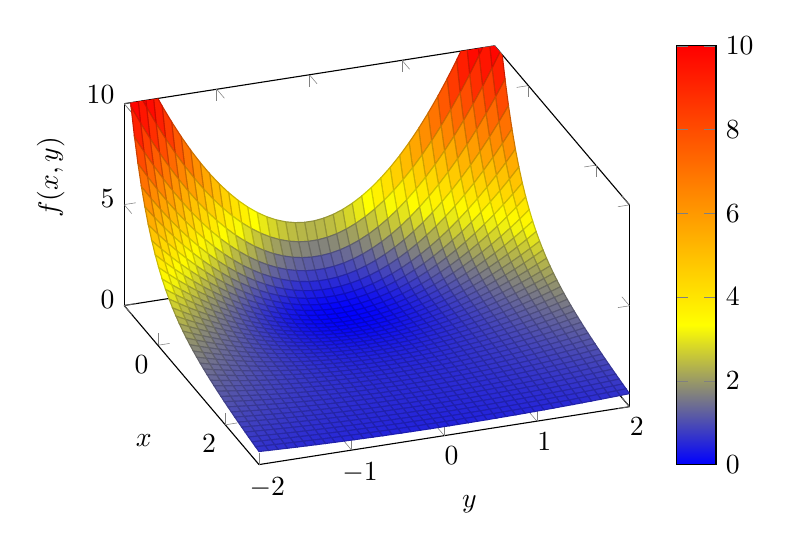
\begin{tikzpicture}
    \begin{axis}[
        width=8cm, % taille du graphique
        view={70}{40}, % angle de vue
        domain=-1:3, y domain=-2:2, % limites pour x et y
        samples=40, % augmenter la résolution du tracé
        xlabel=$x$, ylabel=$y$, zlabel={$f(x, y)$},
        colormap/hot, % palette de couleurs chaudes
        %shader=interp, % ombrage interpolé pour plus de douceur
        colorbar, % ajouter une barre de couleurs
        zmin=0, zmax=10, % étendre les limites de l'axe z
        point meta min=0, point meta max=10, % ajuster la plage de la colormap
    ]
        \addplot3[
            surf, mesh/ordering=y varies % ajouter un maillage
        ]
        {(x^2 + y^2)*exp(-x)};
    \end{axis}
\end{tikzpicture}
}
\end{enumerate}

}